\chapter{Le cloud computing}
\begin{onehalfspace}

\initial{L} e but de ce chapitre est d'exposer le travail fait au niveau de la documentation. Ce chapitre est très riche par des concepts incontournables à la suite de ce rapport. En effet, nous allons commencer par expliquer ce que signifie le cloud concrètement. Ensuite nous présenterons les types de cloud les plus classiques, à savoir IaaS, PaaS et SaaS. Enfin, les notions machines virtuelles et conteneurs seront présentées avec une comparaison détaillée des deux.


\newpage


\section{Le Cloud Computing}

\subsection{Définition}

Le \textbf{Cloud Computing} est l'exploitation de la puissance de calcul ou de stockage de serveurs informatiques distants par l'intermédiaire du réseau internet. Ces serveurs sont loués à la demande selon des critères technique (Bande passante, puissance, etc.). Le cloud computing se caractérise par sa grande souplesse. En effet, il est déstiné aux utilisateurs de tous les niveaux de compétences.

Le cloud est rendu possible grâce à la virtualisation, l'ubiquité des réseaux à grande vitesse, les capacités des navigateurs d'aujourd'hui et l'évolution des piles de développement Web. Avec ces choses en place, il devient moins nécessaire de posséder votre propre infrastructure, ou même de posséder votre propre logiciel. Vous pouvez obtenir ce que vous avez besoin à partir du Cloud, tant que vous en avez besoin.


\subsection{Caractéristiques}

En termes clairs, le Cloud donne la capacité pour les utilisateurs finaux d'utiliser des pièces de ressources. Ces ressources doivent être acquises rapidement et facilement. NIST définit plusieurs caractéristiques qu'il juge essentiel pour qu'un service soit considéré comme «Cloud». Ces caractéristiques comprennent:

\begin{itemize}

\item Service à la demande. La capacité pour un utilisateur final de s' inscrire et recevoir des services sans les longs délais qui ont caractérisé l'informatique traditionnelle;

\item Accessible au réseau large. La Capacité d'accéder au service via les plates-formes standard (bureau, ordinateur portable, mobiles, etc.);

\item La mise en commun des ressources. Les fournisseurs servent plusieurs clients ou «locataires» avec des services provisoires et scalables. Ces services peuvent être ajustés pour répondre aux besoins de chaque client, sans aucune modification apparente pour l'utilisateur;

\item Rapide élasticité. La capacité des ressources doit évoluer pour faire face aux pics de la demande;

\item Service mesuré. La facturation est mesuré et livré


\end{itemize}

Sans ces caractéristiques, l'informatique en nuage n'appore rien par rapport à l'informatique traditionnelle. Une solution Cloud doit démontrer ces caractéristiques et notre projet ne doit pas échapper à cette règle. Dans ce qui suit, nous détaillerons les types classiques du cloud.

\subsection{Les types de Cloud}

Le Cloud Computing est un large terme qui décrit une large collection de services. Dans ce rapport, nous allons expliquer les différents types de services de Cloud communément appelé Software as a Service (SaaS),  Platform as a Service (PaaS) et Infrastructure as a Service (IaaS) et décrirent plus en détails ceux qui touchent à notre sujet.

\begin{figure}[H]
\centering
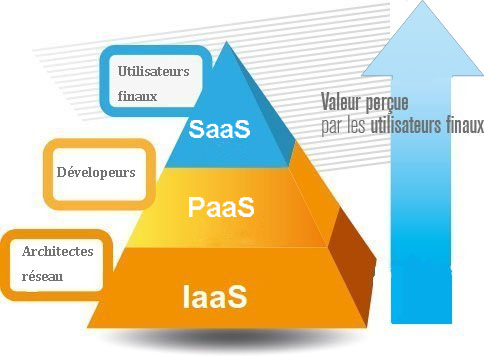
\includegraphics [scale=0.7]{chapitre2/assets/pyramide.jpg}
\caption{Pyramide des services Cloud}
\end{figure}

\subsubsection*{Software as a Service}

La meilleure façon de comprendre ces services est de commencer avec le SaaS, la couche la plus abstraite et celui qu'on utilise peut-être déjà aujourd'hui, même à un niveau personnel. Un exemple simple de SaaS est un service de messagerie en ligne, comme Gmail. Lorsque l'on utilise Gmail, vous n'êtes pas hébergez votre propre serveur de messagerie. C'est Google qui l'héberge, et on est tout simplement entrain d'y accéder via un navigateur comme un client.

SaaS est vraiment orienté vers les utilisateurs finaux de l'entreprise et ne nécéssite pas beaucoup de compétences pour l'utiliser. Le fournisseur décide sur le nombre de ressources à consacrer à l'utilisation de l'application. Le fournisseur décide sur les serveurs, les machines virtuelles, l'équipement de réseau, tout. Enfin, il suffit de pointer le navigateur à l'application.

\subsubsection*{Infrastructure as a Service}

IaaS est à l'autre bout du pyramide du Cloud. Lorsque l'on souhaite garder le contrôle de l'environnement logiciel, mais on veut pas maintenir aucun équipements; Lorsque l'on veut pas acheter des serveurs et de les mettre dans une pièce à température contrôlée ou rien de tout cela; On va chez un fournisseur IaaS et demander tout simplement une machine virtuelle.

L'on peut mettre n'importe quel logiciel que l'on souhaite au-dessus d'IaaS. Sur l'arrière, le fournisseur obtient vous de stockage ou d'autres ressources que l'on a besoin. Ceci est rendu plus facile avec les technologies de virtualisation, qui séparent les ressources physiques de la machine virtuelle qui éxécute le logiciel. IaaS est disponible sur Amazon EC2, GCE de Google et bien d'autres.

L'infrastructure en tant que service ou l'IaaS ne touche pas directement à notre sujet. Du coup, il ne sera mentionné que rarement par la suite.

\subsubsection*{Platform as a Service}

PaaS se situe quelque part entre IaaS et SaaS. Il est pas un produit fini, comme SaaS, encore moins une simple ressource virtuelle vierge, comme IaaS. PaaS est destiné pour les développeurs, il leur donne des outils et des interfaces de haut niveau pour y développer dessus. Par exemple, Windows Azure de Microsoft vous donne des outils pour développer des applications mobiles, des applications sociales, sites Web, jeux et plus encore. Vous construisez ces choses, mais vous utilisez les API et les outils pour les accrocher dans l'environnement Azure et de les exécuter là.


\begin{figure}[H]
\centering
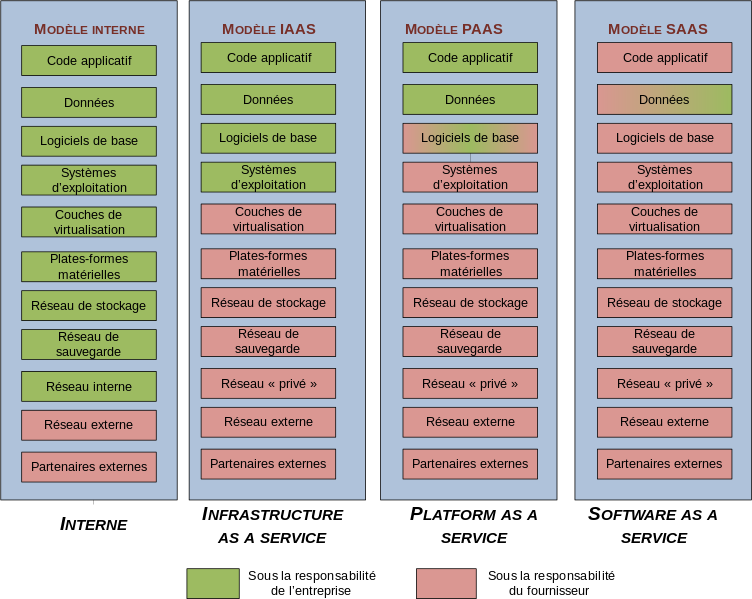
\includegraphics [scale=0.5]{chapitre2/assets/cloud-vs.png}
\caption{L'éxternalisation de l'informatique en Cloud}
\end{figure}


\section{Virtualisation ou containérisation}

\subsection{Virtualisation}

Avec des racines profondément ancrées dans l'informatique, la virtualisation sert à partitionner un seul serveur physique en plusieurs machines virtuelles, comme un espace de stockage ou un réseau, en plusieurs ressources virtuelles. Elle permet une consolidation de serveurs avec une grande souplesse d'utilisation. Dans le contexte de l'informatique en nuage, la virtualisation est importante pour la mise en service et le retrait rapide de serveurs. Ceci étant dit, la scalabilité est la principale caractéristique du Cloud moderne, faute de cela, on ne peut en parler. Ainsi la virtualisation a permis de créer des machines virtuelle, les faire monter en charge à la demande, faire de la migration à chaud, etc. La virtualisation est une technologie permettant d'arriver à une utilisation rentable des serveurs tout en prenant en charge la séparation entre de multiples locataires d'un matériel physique.

Il existe plusieurs solutions de virtualisation, l'on peut citer à titre informatif:

\begin{itemize}
\item VMware, Cette solution, séduisante, pose certains problèmes. En effet, il propose des outils propriétaires et incompatible avec le noyau Linux;
\item Xen est un hyperviseur libre de machines virtuelles, il est considéré comme un outil de virtualisation des plus performants;
\item KVM, Kernel-based Virtual Machine est devenue rapidement la solution de virtualisation de référence pour Linux. Elle est basée sur les architectures Intel ou les architectures AMD;
\item QEMU, est un émulateur machine générique. C'est une solution de virtualisation à utiliser si le processeur de système hôte ne possède pas d'extension matérielle spécifique à la virtualisation.

\end{itemize}

\subsection{Containérisation}

Noyau Linux permet de lancer plusieurs instances isolées de l'espace utilisateur. Un conteneur est un environnement isolé où un ou plusieurs processus peuvent être exécutés. Les conteneurs se concentrent sur l'isolation des processus au lieu d'émuler une machine physique complet.

Historiquement, chroot dans le noyau Linux a fourni un certain niveau d'isolation en fournissant un environnement pour créer et héberger une copie virtualisée d'un logiciel, et ceci depuis le début des années 80. Mais le terme «conteneurs» n'est pas venu jusque vers la fin de l'année 2006. Il a été renommé «Control Groups» (cgroups) pour éviter toute confusion causée par de multiples significations du terme «conteneurs» dans le noyau Linux. «Control Groups est une fonctionnalité du noyau linux qui est disponible depuis la version v2.6.24, elle limite et isole l'utilisation des ressources d'un ensemble de processus. Par la suite, l'isolation de l'espace de noms a été ajouté.

Cela a conduit à l'évolution de Linux Containers (LXC), un environnement de virtualisation au niveau du système d'exploitation qui est construit sur les fonctionnalités du noyau Linux mentionnés plus haut, comme chroot, cgroupes, l'isolation de l'espace de noms, etc.

\subsubsection*{Cgroups}

\begin{itemize}
\item Isolation de l'usage des ressources (CPU, mémoire, E/S, etc.);
\item Limitation des ressources: un groupe peut être configuré pour ne pas dépasser une certaine limite de la mémoire;
\item Priorité: certains groupes peuvent obtenir une plus grande part de CPU ou de débit E/S disque;
\item Mesure de l'usage des ressources;
\item Contrôle: le gel des groupes ou des points de reprise et le redémarrage.
\end{itemize}

\subsubsection*{Namespaces}
\begin{itemize}
\item Partionnement des structures de kernel pour créer des environnements virtuels
\item Des espaces de noms différents

\begin{itemize}
\item pid (processus)
\item net (interfaces réseaux, routage, ...)
\item ipc (communication inter-processus)
\item mnt (points de montage, système de fichiers)
\item uts (Nom de hôte)
\item user (UIDs)
\end{itemize}

\end{itemize}


Contrairement à la virtualisation, la liste des solutions de containérisations n'est pas aussi longue. La plupart d'eux se basent sur ou convergent vers cgroups et namespaces. L'on cite:

\begin{itemize}
\item LXC, Linux containers, combine cgroups et namespace pour fournir un environnement isolé pour les applications;
\item OpenVZ permet de créer multiples conteneurs pour Linux. Dorénavant, tous les efforts des développeurs d'OpenVZ vont aller dans le sens de fusionner les fonctionnalités d'OpenVZ avec LXC;
\item lmctfy, Let Me Contain That For You, est une solution open source de containérisation de Google qui est basé sur cgroups. Le futur de lmctfy est flou vu que Google avait commencé à migrer les concepts de lmctfy vers Docker;
\item Docker, ce n'est pas une autre solution, mais il est basé sur LXC et fournit une couche de haut niveau accessible pour l'utilsateur;

\end{itemize}

\subsection{Etude comparative}

Le choix de la solution a été proposé fortement par la société. On a opté pour une solution de containérisation (Docker) dans la mesure où un benchmark prouve son efficacité et sa légèreté.


\begin{figure}[H]
\centering
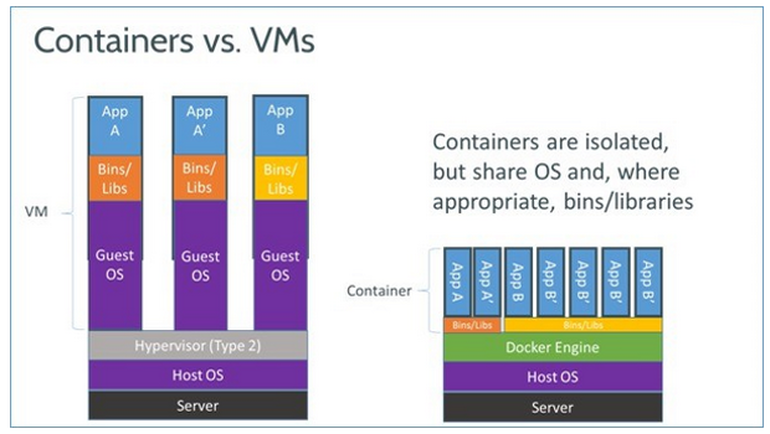
\includegraphics [scale=0.5]{chapitre2/assets/vm-container.png}
\caption{Virtualisation VS Containérisation}
\end{figure}


Dans la containérisation, ou la virtualisation au niveau du système d'exploitation, l'hôte et les invités partagent le même noyau. Cette approche réduit le gaspillage de ressources puisque chaque conteneur contient uniquement l'application et les bibliothèques et les binaires nécéssaires. Le rôle de l'hyperviseur est assurée par un moteur léger de la containérisation comme Docker, qui est installé au-dessus du système d'exploitation hôte.

Le principal avantage des conteneurs c'est qu'ils sont libres de l'overhead du système d'exploitation contrairement aux machines virtuelles, ce qui leur rend considérablement plus légers, plus faciles à télécharger ainsi que plus rapides à lancer. Cet avantage permet également un serveur d'héberger potentiellement beaucoup plus de conteneurs que de machines virtuelles. Scalabilité, portabilité, facilité de déploiement sont quelques avantages.


Lors de cette étude, nous allons se baser sur un travail réalisé par IBM\cite{ibm-benchmark-docker}, où nous allons mettre l'accent sur les la différence des performances entre Docker et KVM. Le benchmark concerne 15 machines virtuelles simultanément en marche sous OpenStack.

{\rowcolors{1}{tabOdd}{tabEven}
\begin{center}
\begin{table}[H]

	\caption{Performances: Docker VS KVM \label{tab:table_label}}
	\begin{tabular}{| c | c | c |} 


	\hline
	\rowcolor{tabHead}
	\textbf{Tests} & \textbf{Docker} & \textbf{KVM}\\ [0.95ex] 
	\hline\hline
	Temps moyen de démarrage 					& 3.9s 				& 	5.88s \\ 
	\hline\hline
	Usage CPU démarrage (sys)					& 0.44\%			& 	2.08\% \\ 
	\hline\hline
	Usage CPU démarrage (usr)					& 1.14\% 			& 	12.6\% \\ 
	\hline\hline
	Usage de mémoire au démarrage				& 45.8Mb/VM 		& 	185Mb/VM \\ 
	\hline\hline

	Temps moyen de redémarrage 					& 2.54s 			& 	124.45s \\ 
	\hline\hline
	Usage CPU redémarrage (sys)					& 0.11\% 			& 	0.19\% \\ 
	\hline\hline
	Usage CPU redémarrage (usr)					& 0.34\% 			& 	0.82\% \\ 
	\hline\hline
	Usage de mémoire au redémarrage				& 57Mb	 			& 	467Mb	  \\ 
	\hline\hline

	Temps moyen de suppression 					& 4.09s 			& 	4.45s \\ 
	\hline\hline

	Temps moyen de Snapshot (VM to Image) 		& 26.39s 			& 	42.93s \\ 
	\hline\hline
	Usage CPU de Snapshot (sys)			 		& 0.11\% 			& 	1.07\% \\ 
	\hline\hline
	Usage CPU de Snapshot (usr)			 		& 0.4\% 			& 	1.58\% \\ 
	\hline\hline
	Usage de mémoire de Snapshot		 		& 48Mb 				& 	114Mb \\ 
	\hline\hline

	Usage de mémoire état stable				& 3.52s 			& 	5.87s \\ 
	\hline\hline

	Calcul des nombres premier jusqu'à 20000	& 15.11s 			& 	15.08s \\ 
	\hline\hline

	Débit du réseaux (Mbits/s)					& 940.26 			& 	940.56 \\ 
	\hline
	\end{tabular}
\end{table}
\end{center}
}


\begin{figure}[H]
\centering
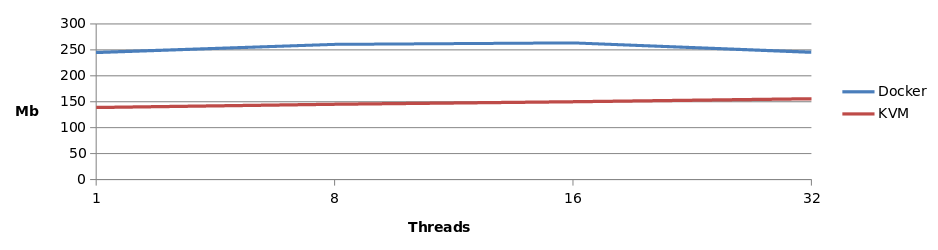
\includegraphics [width=160mm]{chapitre2/assets/file-io-read.png}
\caption{Lecture du disque dur}
\label{fig:}
\end{figure}

\begin{figure}[H]
\centering
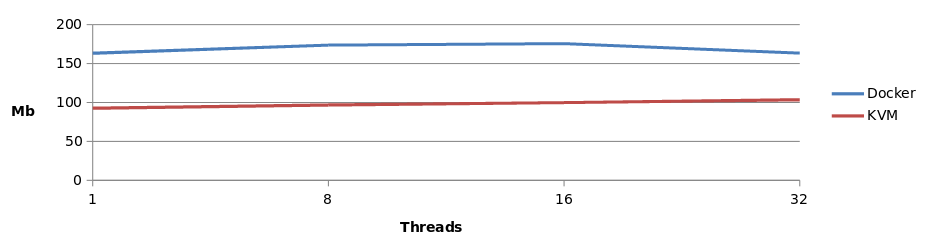
\includegraphics [width=160mm]{chapitre2/assets/file-io-write.png}
\caption{Ecriture dans le disque dur}
\label{fig:}
\end{figure}


En somme, il va s'en dire que Docker l'emporte largement par rapport à KVM, tant qu'en termes de la gestion des ressources (CPU, RAM) qu'en termes du temps consommé pour le démarrage, le redémarrage et la suppression. Par ailleurs, Docker est le meilleur dans lecture/écriture dans le disque dur et s'approche à des performances natives. Ainsi, Il serait donc judicieux de virtualiser les bases de données dans des conteneurs que dans des machines virtuelles. 







\section{L'outil Docker}
\subsection{Présentation de Docker}
Docker est un logiciel open source qui automatise le déploiement d'applications dans des conteneurs logiciels. C'est un outil qui peut empaqueter une application et ses dépendances dans un conteneur virtuel, qui pourra être exécuté sur n'importe quel serveur Linux ou Windows (Boot2Docker). En fait, Docker a pour objectif de \textbf{faciliter le déploiement d’applications}, d’avoir plusieurs versions d’une même application sur un son serveur (phase de développement, tests), mais aussi d’\textbf{automatiser le packaging d’applications}. Avec Docker, on s’oriente vers de l’intégration et du déploiement en continu grâce au système de container. De plus, Docker permet de garder son système de base propre, tout en installant de nouvelles fonctionnalités au sein de containers, on part d’une base qui est le système d’exploitation et on ajoute différentes briques conteneurisées. Docker a été distribué en tant que projet open source à partir de mars 2013.
\begin{figure}[H]
\centering
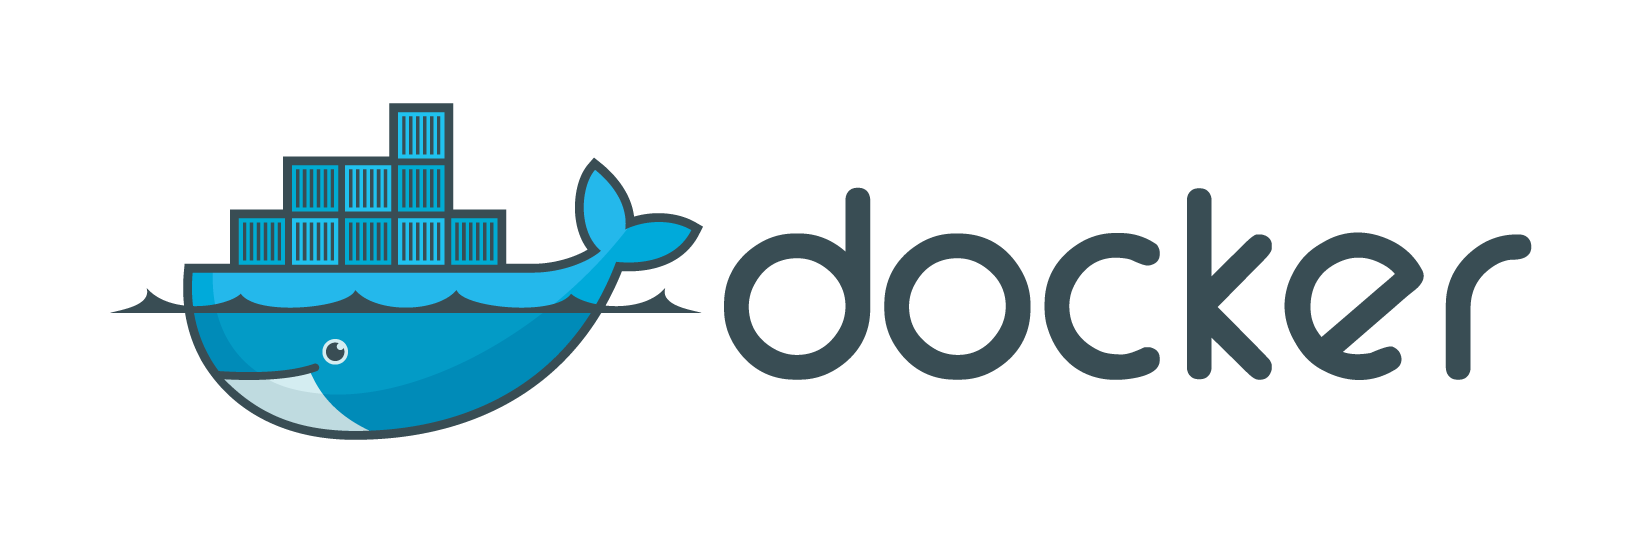
\includegraphics [scale=0.5]{chapitre2/assets/docker.png}
\caption{Logo de Docker}
\end{figure}

\subsection{Utilisation de Docker}
Docker propose de nombreux templates qui permettent de déployer des applications en container, très rapidement. La communauté est très active, ce qui permet aux utilisateurs de disposer de nombreux containers applicatifs préfaits.
Docker est basé sur LXC (Linux Containers) qui est une référence sous Linux quant à l’utilisation des containers. Par ailleurs, Docker intègre les éléments suivants :
\begin{itemize}
\item \textbf{Control Groups} : Fonctionnalité du noyau Linux pour limiter, compter et isoler les ressources (CPU, RAM, etc.) utilisées par un groupe de processus.
\item \textbf{AppArmor et SElinux} : Gestion avancée des permissions aussi bien au niveau des applications qu’au niveau du système de fichiers.
\item \textbf{Kernel namespace} : Fonctionnalité du noyau Linux qui permet l’isolation, afin de s’assurer qu’un container ne puisse pas en affecter un autre.
\item \textbf{chroot} : Fonctionnalité qui permet de changer la racine d’un processus, afin de l’isoler sur un système par mesure de sécurité.
\end{itemize}

Docker propose des services pour effectuer facilement différentes actions : créer, éditer, publier et exécuter des containers. On parlera souvent des notions de containers, images et dockerfiles.

\begin{itemize}
\item \textbf{DockerFile} : Fichier source qui contient les instructions, éléments à installer, c’est un fichier de configuration.
\item \textbf{Image} : Compilation d’un fichier DockerFile pour former une image portable, prête à être déployée.
\item \textbf{Container} : Exécution d’une image, mise en container d’une image.
\end{itemize}


Le schéma suivant décrit le fonctionnement de l'outil \emph{Docker}: 
\begin{figure}[H]
\centering
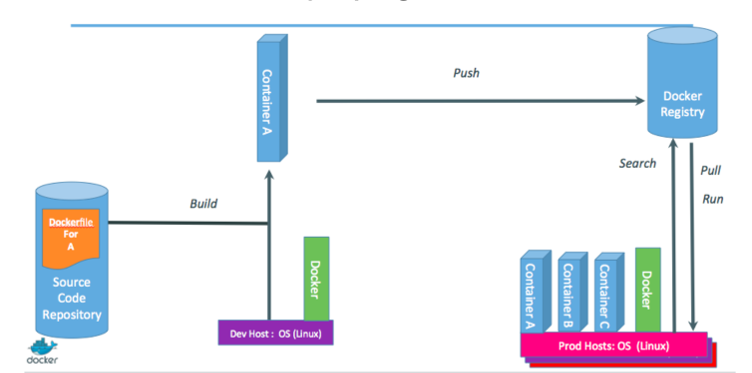
\includegraphics [scale=0.6]{chapitre2/assets/utilisation.png}
\caption{Fonctionnement de Docker}
\end{figure}

\end{onehalfspace}
\label{table:} % is used to refer this table in the text
